%%%%%%%%%%%%%%%%%%%% CHAPTER 3 %%%%%%%%%%%%%%%%%%%%%%%%%%
%%%%% Variables and Operators %%%%%%%%%%%%%%%%%%%%%%%%%%%%%%%%%%% 
\section{Simultaneous Non-Linear Systems of Equations}
Non-linear systems are extensions of the linear systems cases except the systems involve products and powers of the unknown variables.
Non-linear problems are often quite difficult to manage, especially when the systems are large (many rows and many variables).

The solution to non-linear systems, if non-trivial yet alone even possible, are iterative.  

Within the iterative steps is a linearization component -- these linear systems which are intermediate computations within the overall solution process are treated by an appropriate linear system method (direct or iterative). 

In \textbf{R} it is sometimes successful to solve by the nonlinear minimization tool built-in, but neither efficient, nor particularly useful when the system gets large. On the \texttt{CRAN} there are a couple of packages devoted to non-linear systems, and these would be reasonable places to consider.

In this chapter we will illustrate an iterative technique called Quasi-Linearization, and the next chapter we will formally extend Newton's method to multi-dimensional cases.

%%%%%%%%%%%%%%%%%%%%%%%%%%%%%%%%%%%%%%%%%%%%%%%%%%%%%%%%%%%%%%%'
\begin{gather}
\begin{matrix}
x^2 & +~y^2  \\
 e^x & +~y  \\
\end{matrix}
\begin{matrix}
= 4\\
= 1\\
\end{matrix}
\end{gather}

Suppose we have a solution guess $x_{k},y_{k}$, which of course could be wrong, but we could linearize about that guess as

\begin{gather}
\mathbf{A} =
\begin{pmatrix}
x_k & + ~y_k  \\
0 & + ~1  \\
\end{pmatrix}
~\mathbf{x} = 
\begin{pmatrix}
x_{k+1} \\
y_{k+1} \\
\end{pmatrix}
~ \mathbf{b} = 
\begin{pmatrix}
4\\
1 - e^{x_k}\\
\end{pmatrix}
\end{gather}

Now the system is linear, and we can solve for $\mathbf{x_{k+1}}$ much like the Jacobi iteration of the previous chapter.  If the system is convergent (not all are) then we update in the same fashion, and repeat until complete.

Listing \ref{lst:QuasiLinear} is a script that implements the quasi-linearization method.  
The starting vector is crucial, and the next several screen captures illustrate good starting vectors (resulting in a solution) and poor ones.
\newpage
\begin{lstlisting}[caption=R code demonstrating Non-Linear by quasi-linearization , label=lst:QuasiLinear]
# R script to solve non-linear example by quasi-linearization
Amat <- matrix(0,nrow=2,ncol=2)
Brhs <- numeric(0)
x_guess <- c(-1.9, 0.8)
maxiter <- 20
message("Initial Guess"); print(x_guess); message("Original Equations - x_guess "); 
message( x_guess[1]^2 + x_guess[2]^2, " : should be 4 ")
message( exp(x_guess[1]) + x_guess[2], " : should be 1 ")
# Construct the current quasi-linear model
for (iter in 1:maxiter){
Amat[1,1] <- x_guess[1]; Amat[1,2] <- x_guess[2];
Amat[2,1] <- 0         ; Amat[2,2] <- 1;
Brhs[1] <- 4
Brhs[2] <- 1-exp(x_guess[1])
# Solve for the new guess
x_new <- solve(Amat,Brhs)
# Update
x_guess <- x_new
}
print(Amat); print(Brhs);
message("Current Guess"); print(x_new)
message("Original Equations - x_new")
message( x_new[1]^2 + x_new[2]^2, " : should be 4 ")
message( exp(x_new[1]) + x_new[2], " : should be 1 ")
\end{lstlisting}

Figure \ref{fig:QuasiLinear-Works1} is a screen capture of the algorithm started near a solution, that sort-of converges to the solution.  Not really satisfying, but at least not divergent.

\begin{figure}[h!] %  figure placement: here, top, bottom, or page
   \centering
   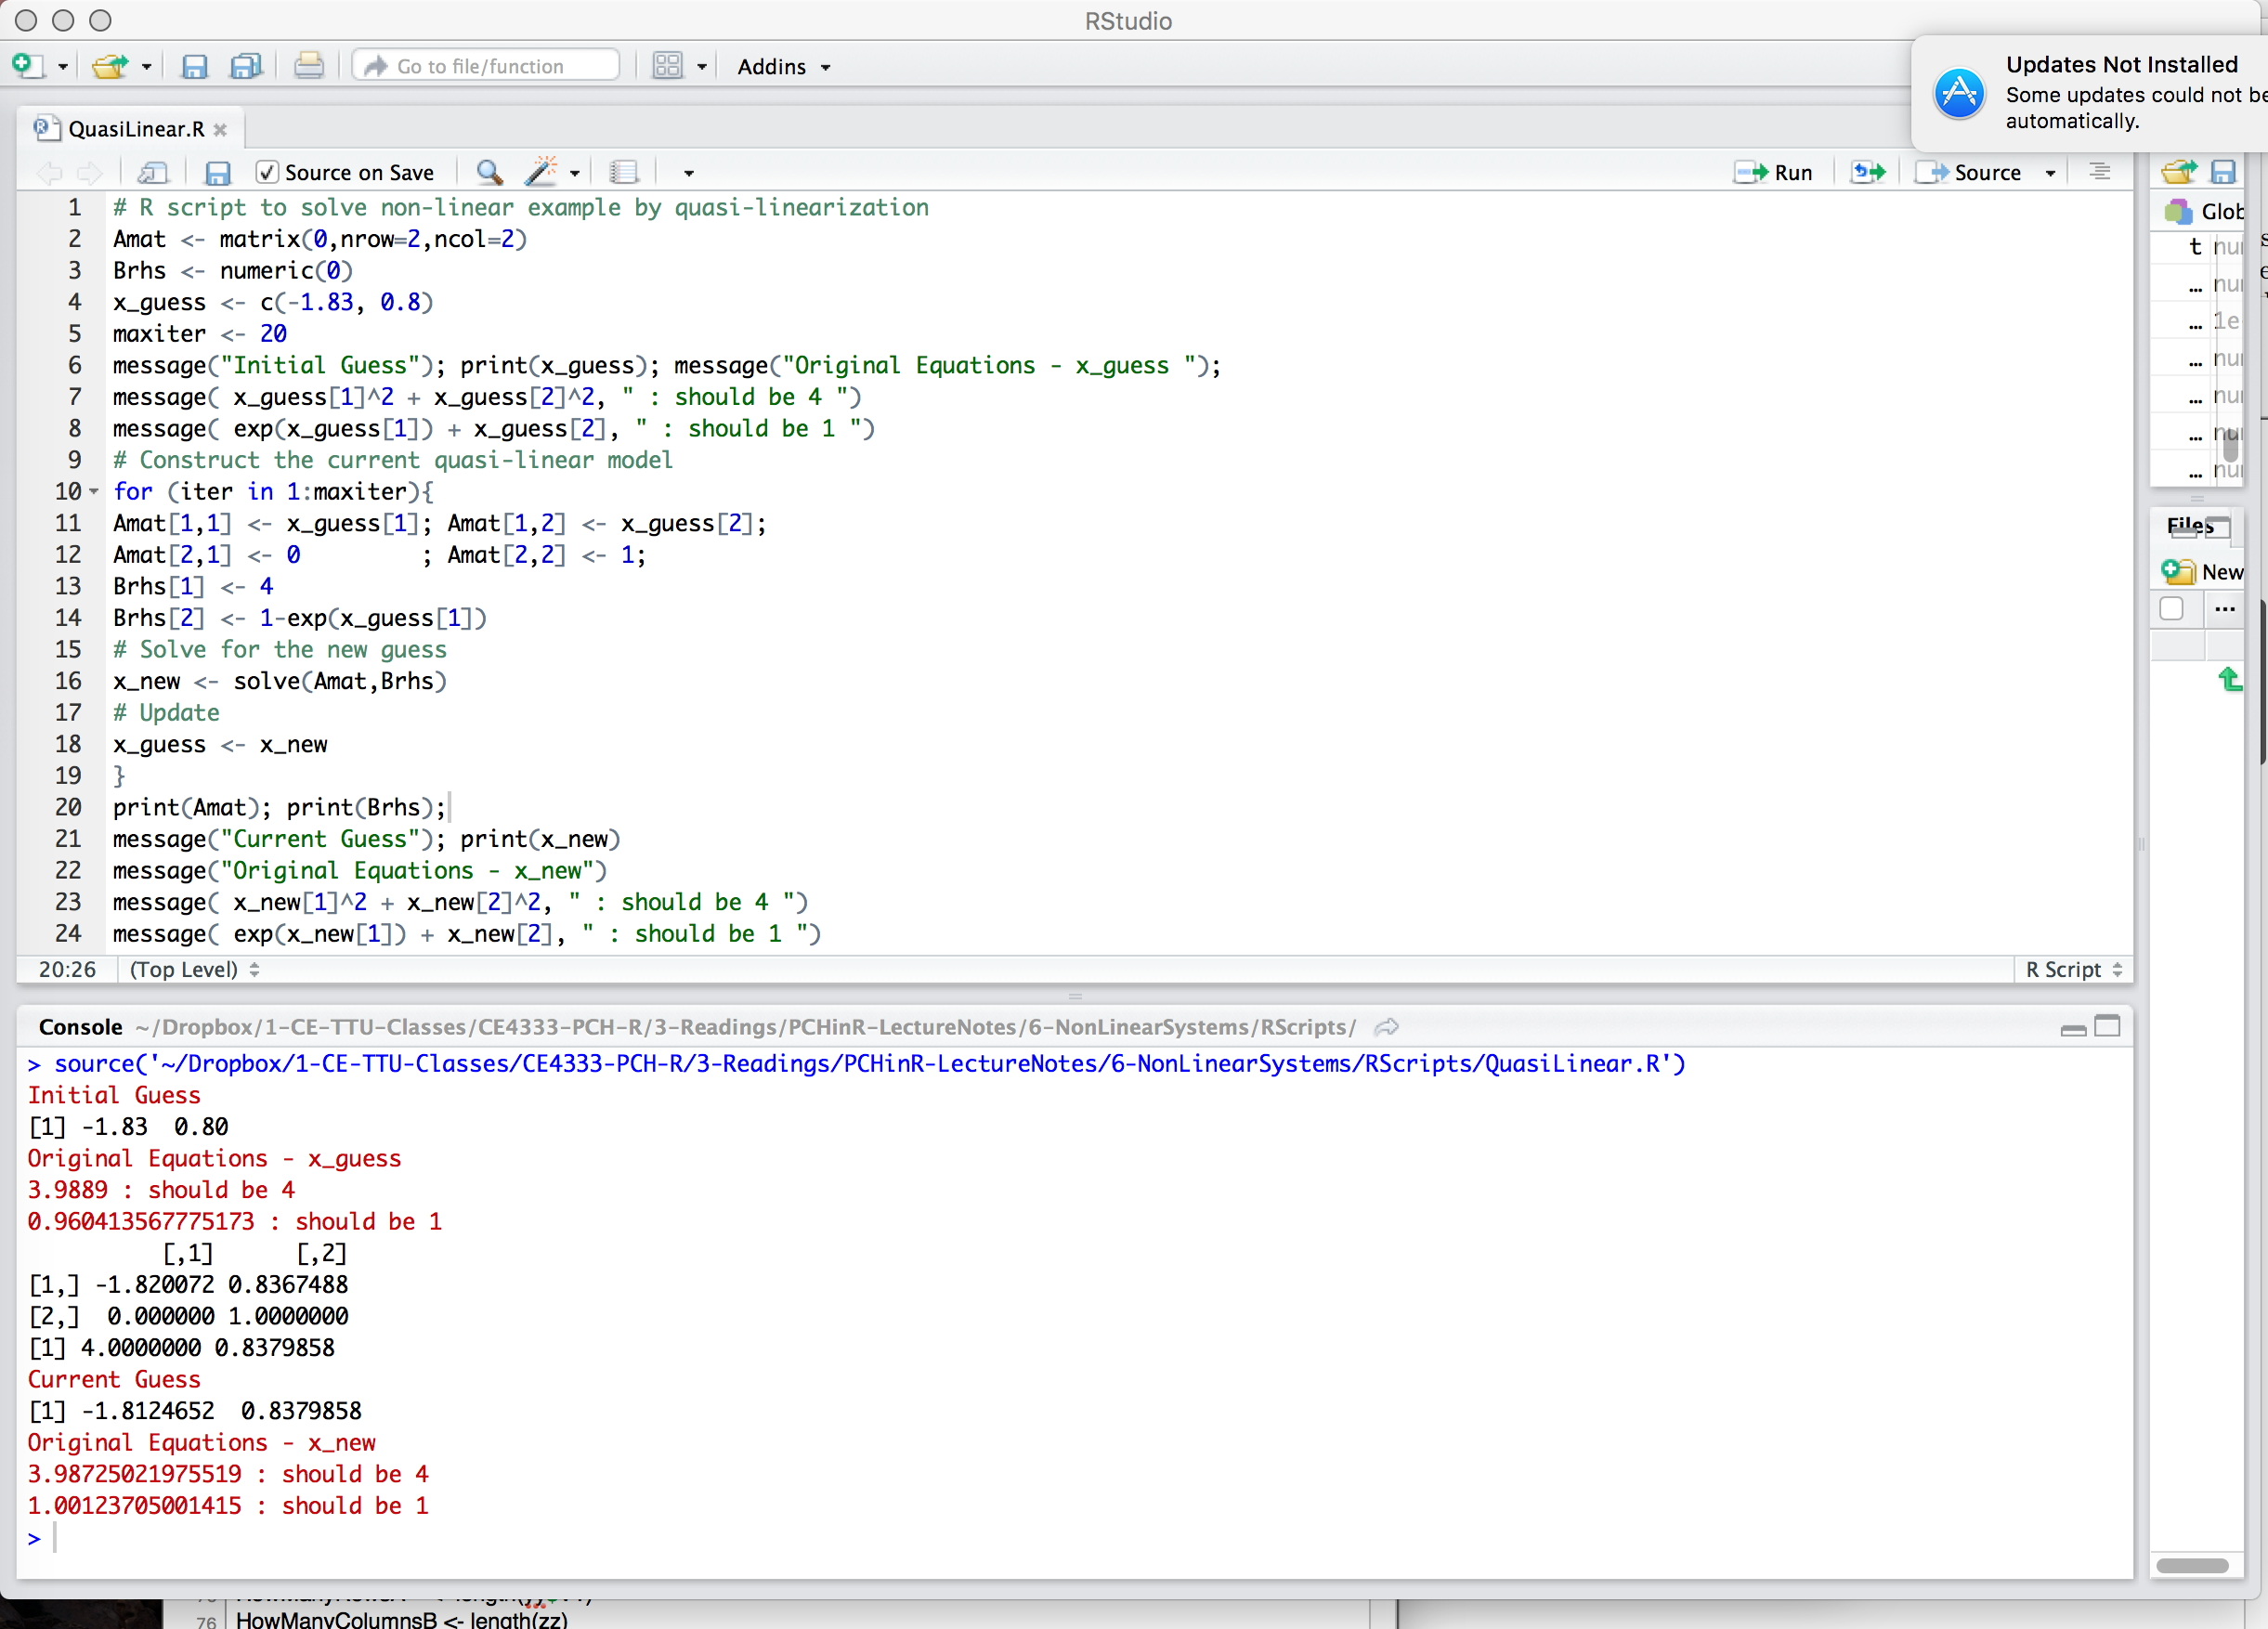
\includegraphics[width=6in]{./6-NonLinearSystems/QuasiLinear-Works1.jpg} 
   \caption{Quasi-linear, started near a solution, converges (sort-of) to the solution}
   \label{fig:QuasiLinear-Works1}
\end{figure}
\clearpage

Figure \ref{fig:QuasiLinear-Fail1} is a screen capture of the algorithm started near a solution, that fails to converge --- it actually diverged.

\begin{figure}[h!] %  figure placement: here, top, bottom, or page
   \centering
   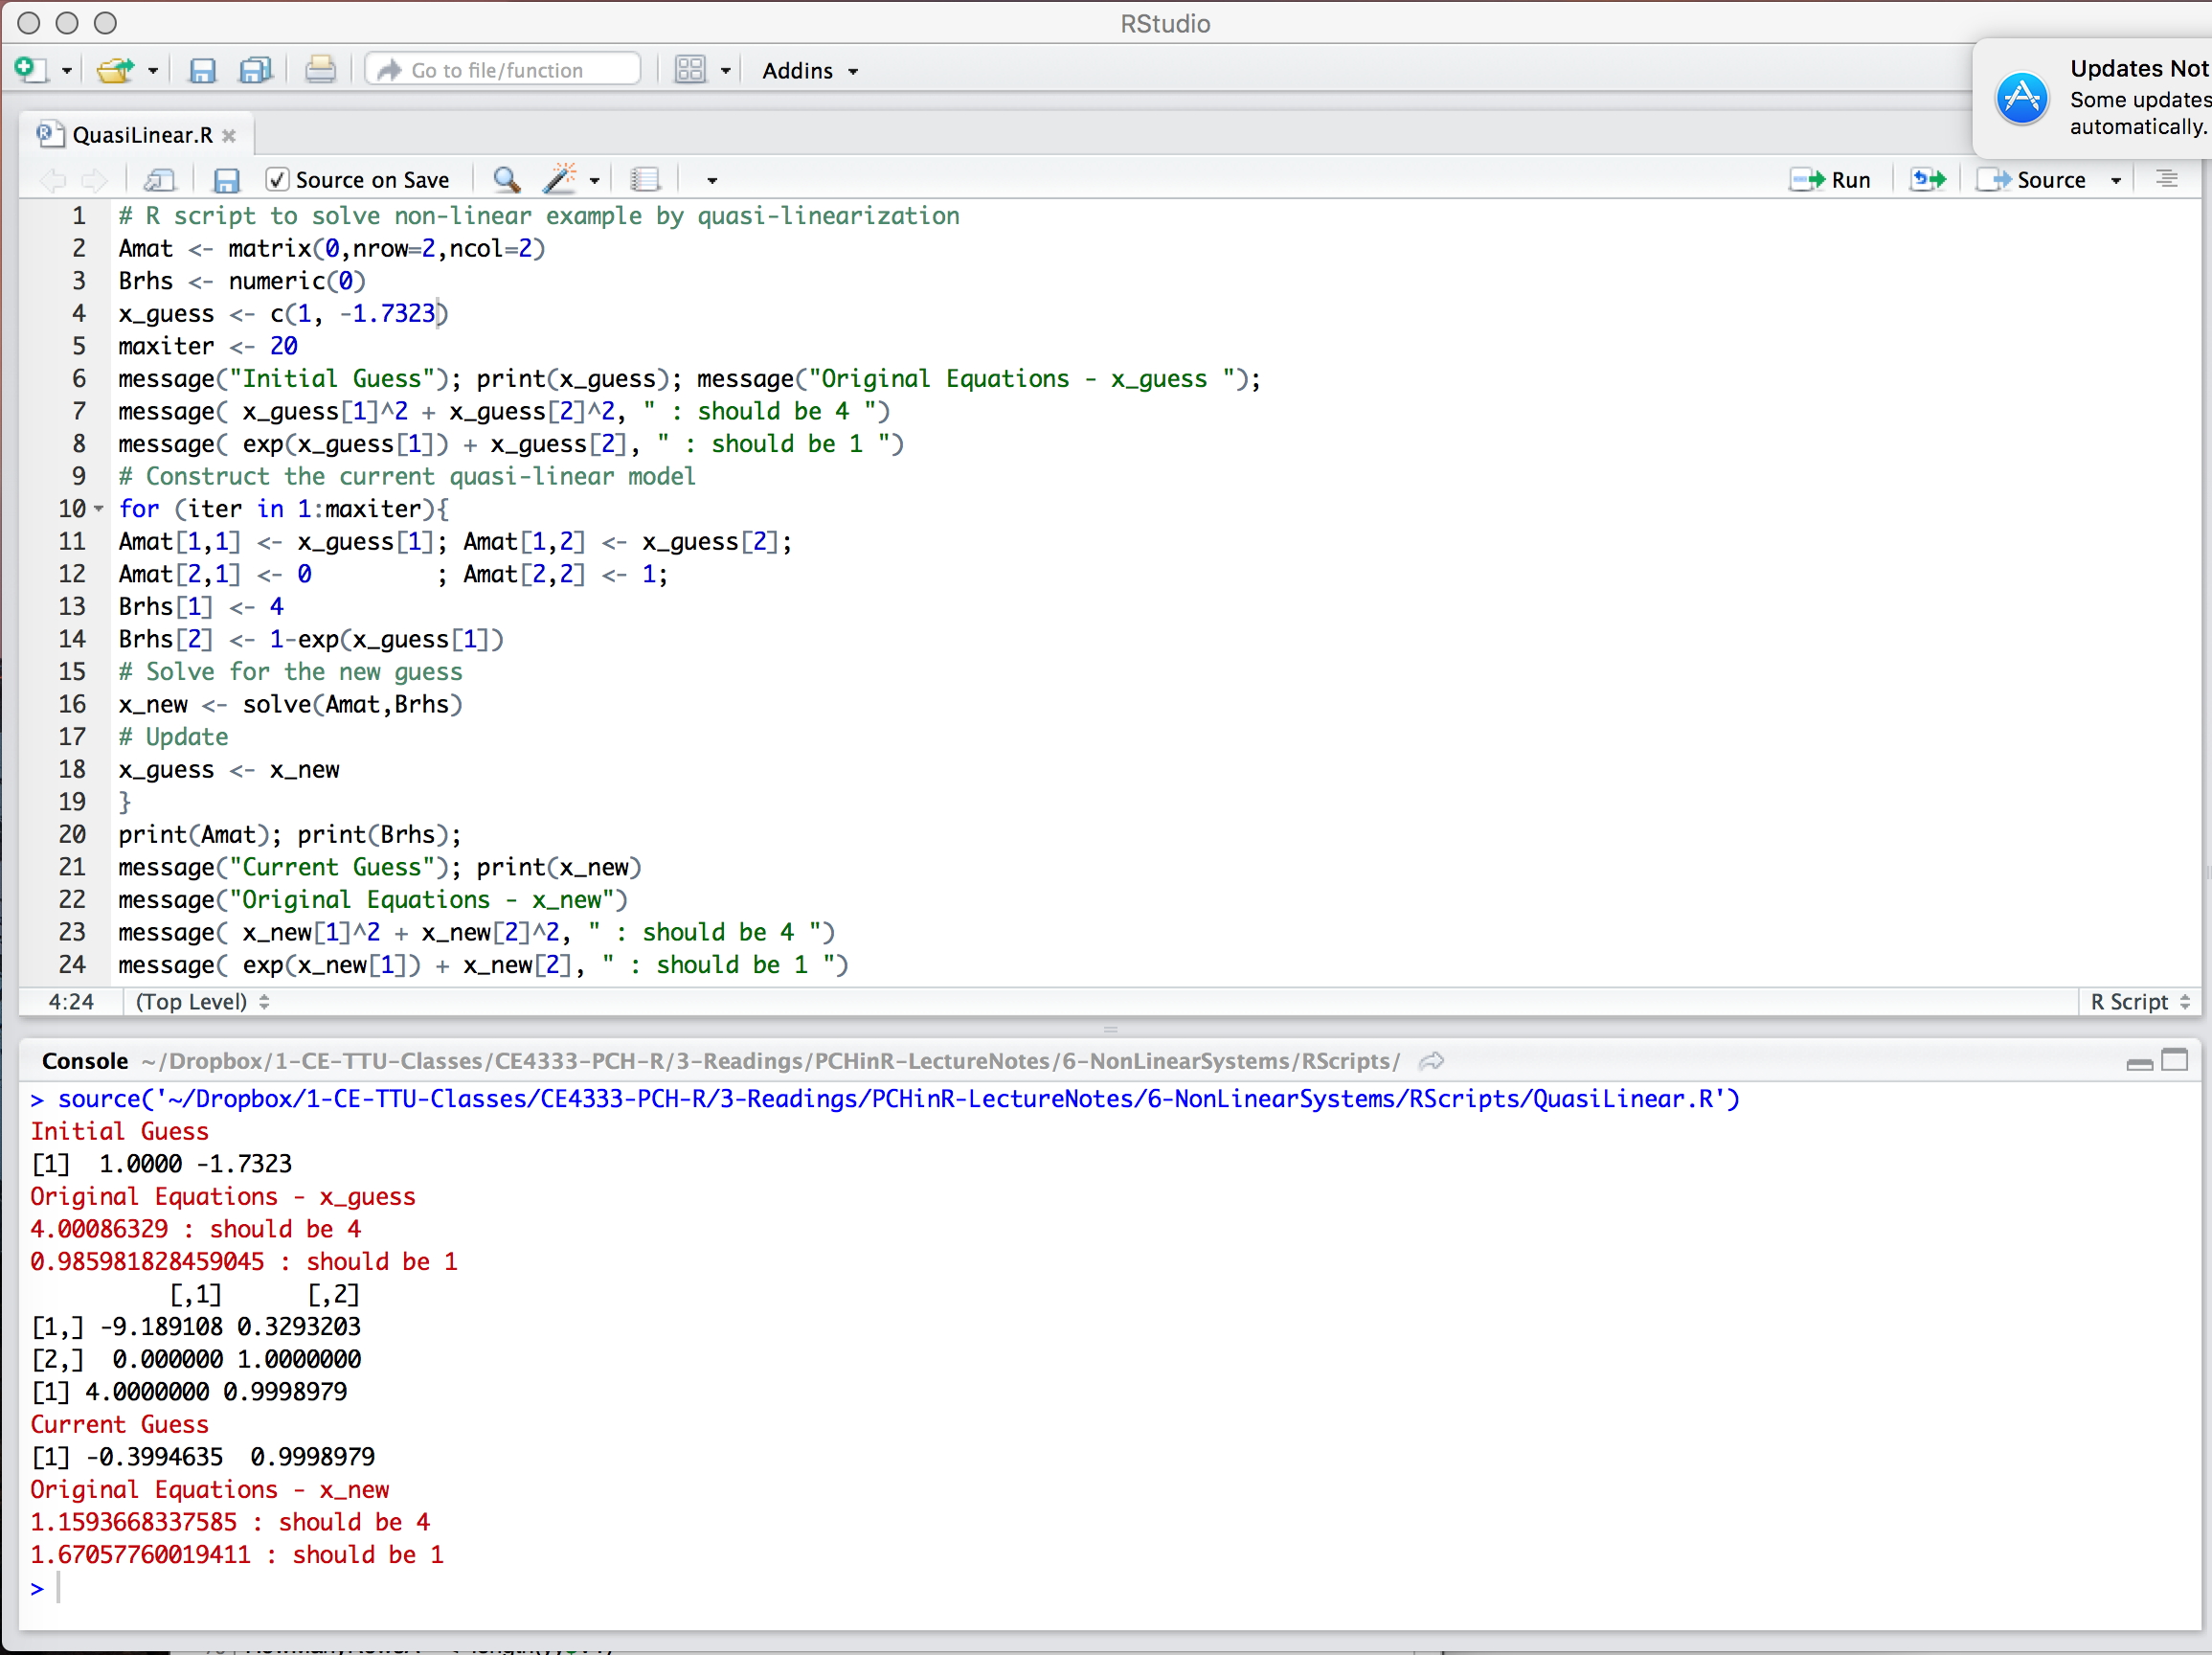
\includegraphics[width=6in]{./6-NonLinearSystems/QuasiLinear-Fail1.jpg} 
   \caption{Quasi-linear, started near a solution, fails to converge}
   \label{fig:QuasiLinear-Fail1}
\end{figure}

What is really needed is a much more reliable algorithm.  
Sometimes the non-linear minimization tools can successfully be used.  
We will try that next.

Lets restructure our equation system a bit into

\begin{gather}
\mathbf{f(x)} = 
\begin{matrix}
f_1(x,y) = & x^2 & +~y^2 & - 4\\
f_2(x,y) = & e^x & +~y  & - 1\\
\end{matrix}
\end{gather}

At the solution $\mathbf{x}$, the result should be $\mathbf{f(x) = 0}$.  
But if we are not at a solution, then the result will be non-zero (and represents the error) --- one tool we have is a non-linear minimization tool in \textbf{R} that can minimize functions.  
So now we need the sum-of-squared errors, which with vectors is simply the inner product of the vector with itself:

\begin{equation}
\mathbf{F(x)} = \mathbf{f(x)}^T \cdot \mathbf{f(x)}
\end{equation}

So lets rewrite the script to construct $\mathbf{f(x)}$ and $\mathbf{F(x)}$, then implement the non-linear minimizer, \texttt{nlm(\dots)} in \textbf{R}.   Listing \ref{lst:Minimize} is a listing that implements these changes.  Notice the two prototype functions, the first takes vector input and returns vector output --- internal (to the function) definition of a vector using \texttt{func <- numeric(0)} provides the memory space in the program.\footnote{If you get an error message with the words \texttt{... Atomic ....}, it means that something in a function is trying to address a variable for which there is no space, or trying to address a global (external to the function) variable directly.  These are pretty hard errors to debug (fix), so I have gotten into the habit of building and testing the prototype functions before I even try to get the rest of the program to run.}

\begin{lstlisting}[caption=R code demonstrating Non-Linear by Minimization , label=lst:Minimize]
# R script for system of non-linear equations using minimization
# WARNING -- This is not recomended for large systems
# forward define the functions
####### f(x) #################
func <- function(x_vector){
  func <- numeric(0)
  func[1] <- x_vector[1]^2 + x_vector[2]^2 - 4
  func[2] <- exp(x_vector[1]) + x_vector[2] - 1
  return(func)
}
######### F(x) ###############
bigF <- function(x_vector){
  vector <- numeric(0)
  vector <- func(x_vector)
  bigF <- t(vector) \%*\% vector
  return(bigF)
}
#############################
# forward define some variables
# starting guess
x_guess <- c(1,-1.7)
result <- nlm(bigF,x_guess)
message(" Estimated bigF Value : ",result$minimum)
message(" Estimated x_vector Value : ")
print(result$estimate)
message(" Estimated func Value : ")
print(func(result$estimate))
\end{lstlisting}

Figure \ref{fig:NLM-Method-Works} is a screen capture of the script for the first solution to the system of equations, we have started quite close to a solution and the method converges to the correct solution.  The object named \texttt{result} contains several items of which we have only accessed two.  Notice how we have addressed these items using the \texttt{name\$attribute} method.

Figure \ref{fig:NLM-Method-Works2} is a screen capture of the script for the second solution to the system of equations, we have started quite close to a solution and the method converges to the correct solution.  

Naturally, to be really useful we should test the method for starting values relatively far from the solution; Figure \ref{fig:NLM-Method-Works3} is a screen capture of such testing for a few different start vectors. 
Observe that the solution at (-1.8,0.8) is the preferred solution in most cases unless we start very close to the second solution at (1,-1.7).  
This kind of preference to one solution over another is quite common in non-linear systems (sometimes these particular solutions are called attractors).
The related observation is that we can find starting vectors that simply fail --- this phenomenon is also quite common (sometimes called sensitive dependence on initial conditions).

\begin{figure}[h!] %  figure placement: here, top, bottom, or page
   \centering
   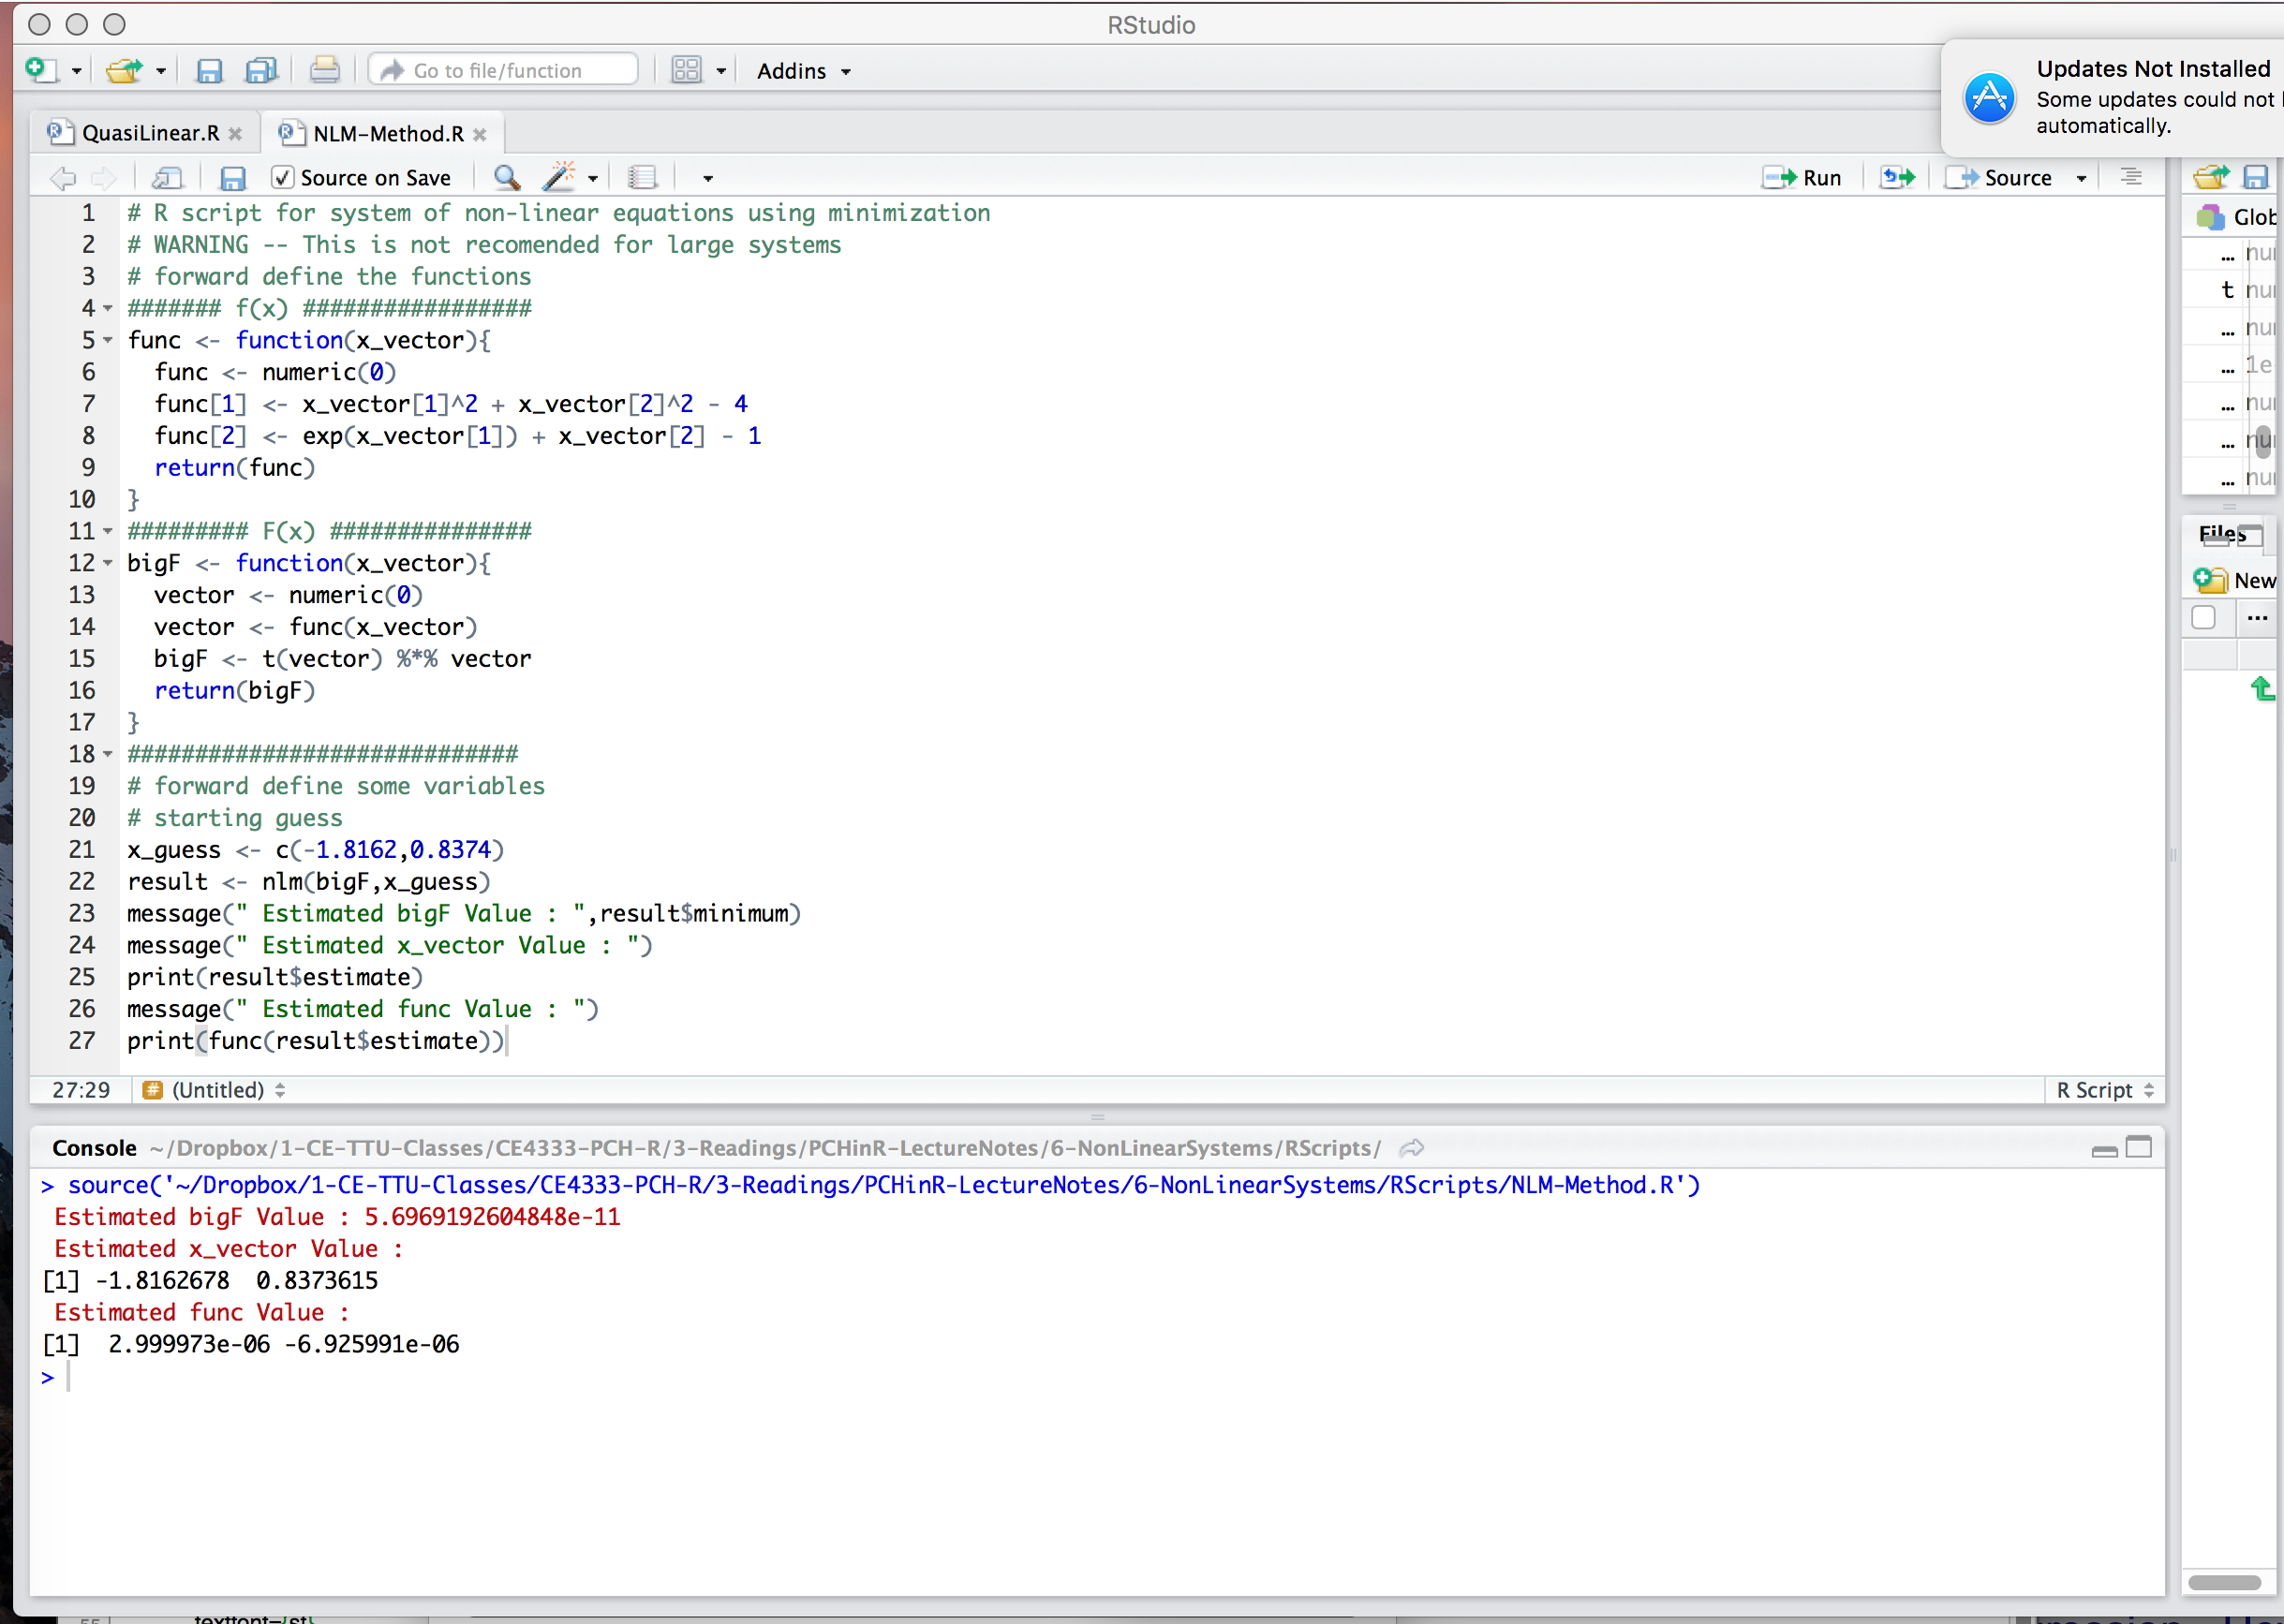
\includegraphics[height=4in]{./6-NonLinearSystems/NLM-Method-Works.jpg} 
   \caption{Solution using \texttt{nlm(\dots)}.  Start vector (-1.8,0.8)}
   \label{fig:NLM-Method-Works}
\end{figure}
\begin{figure}[h!] %  figure placement: here, top, bottom, or page
   \centering
   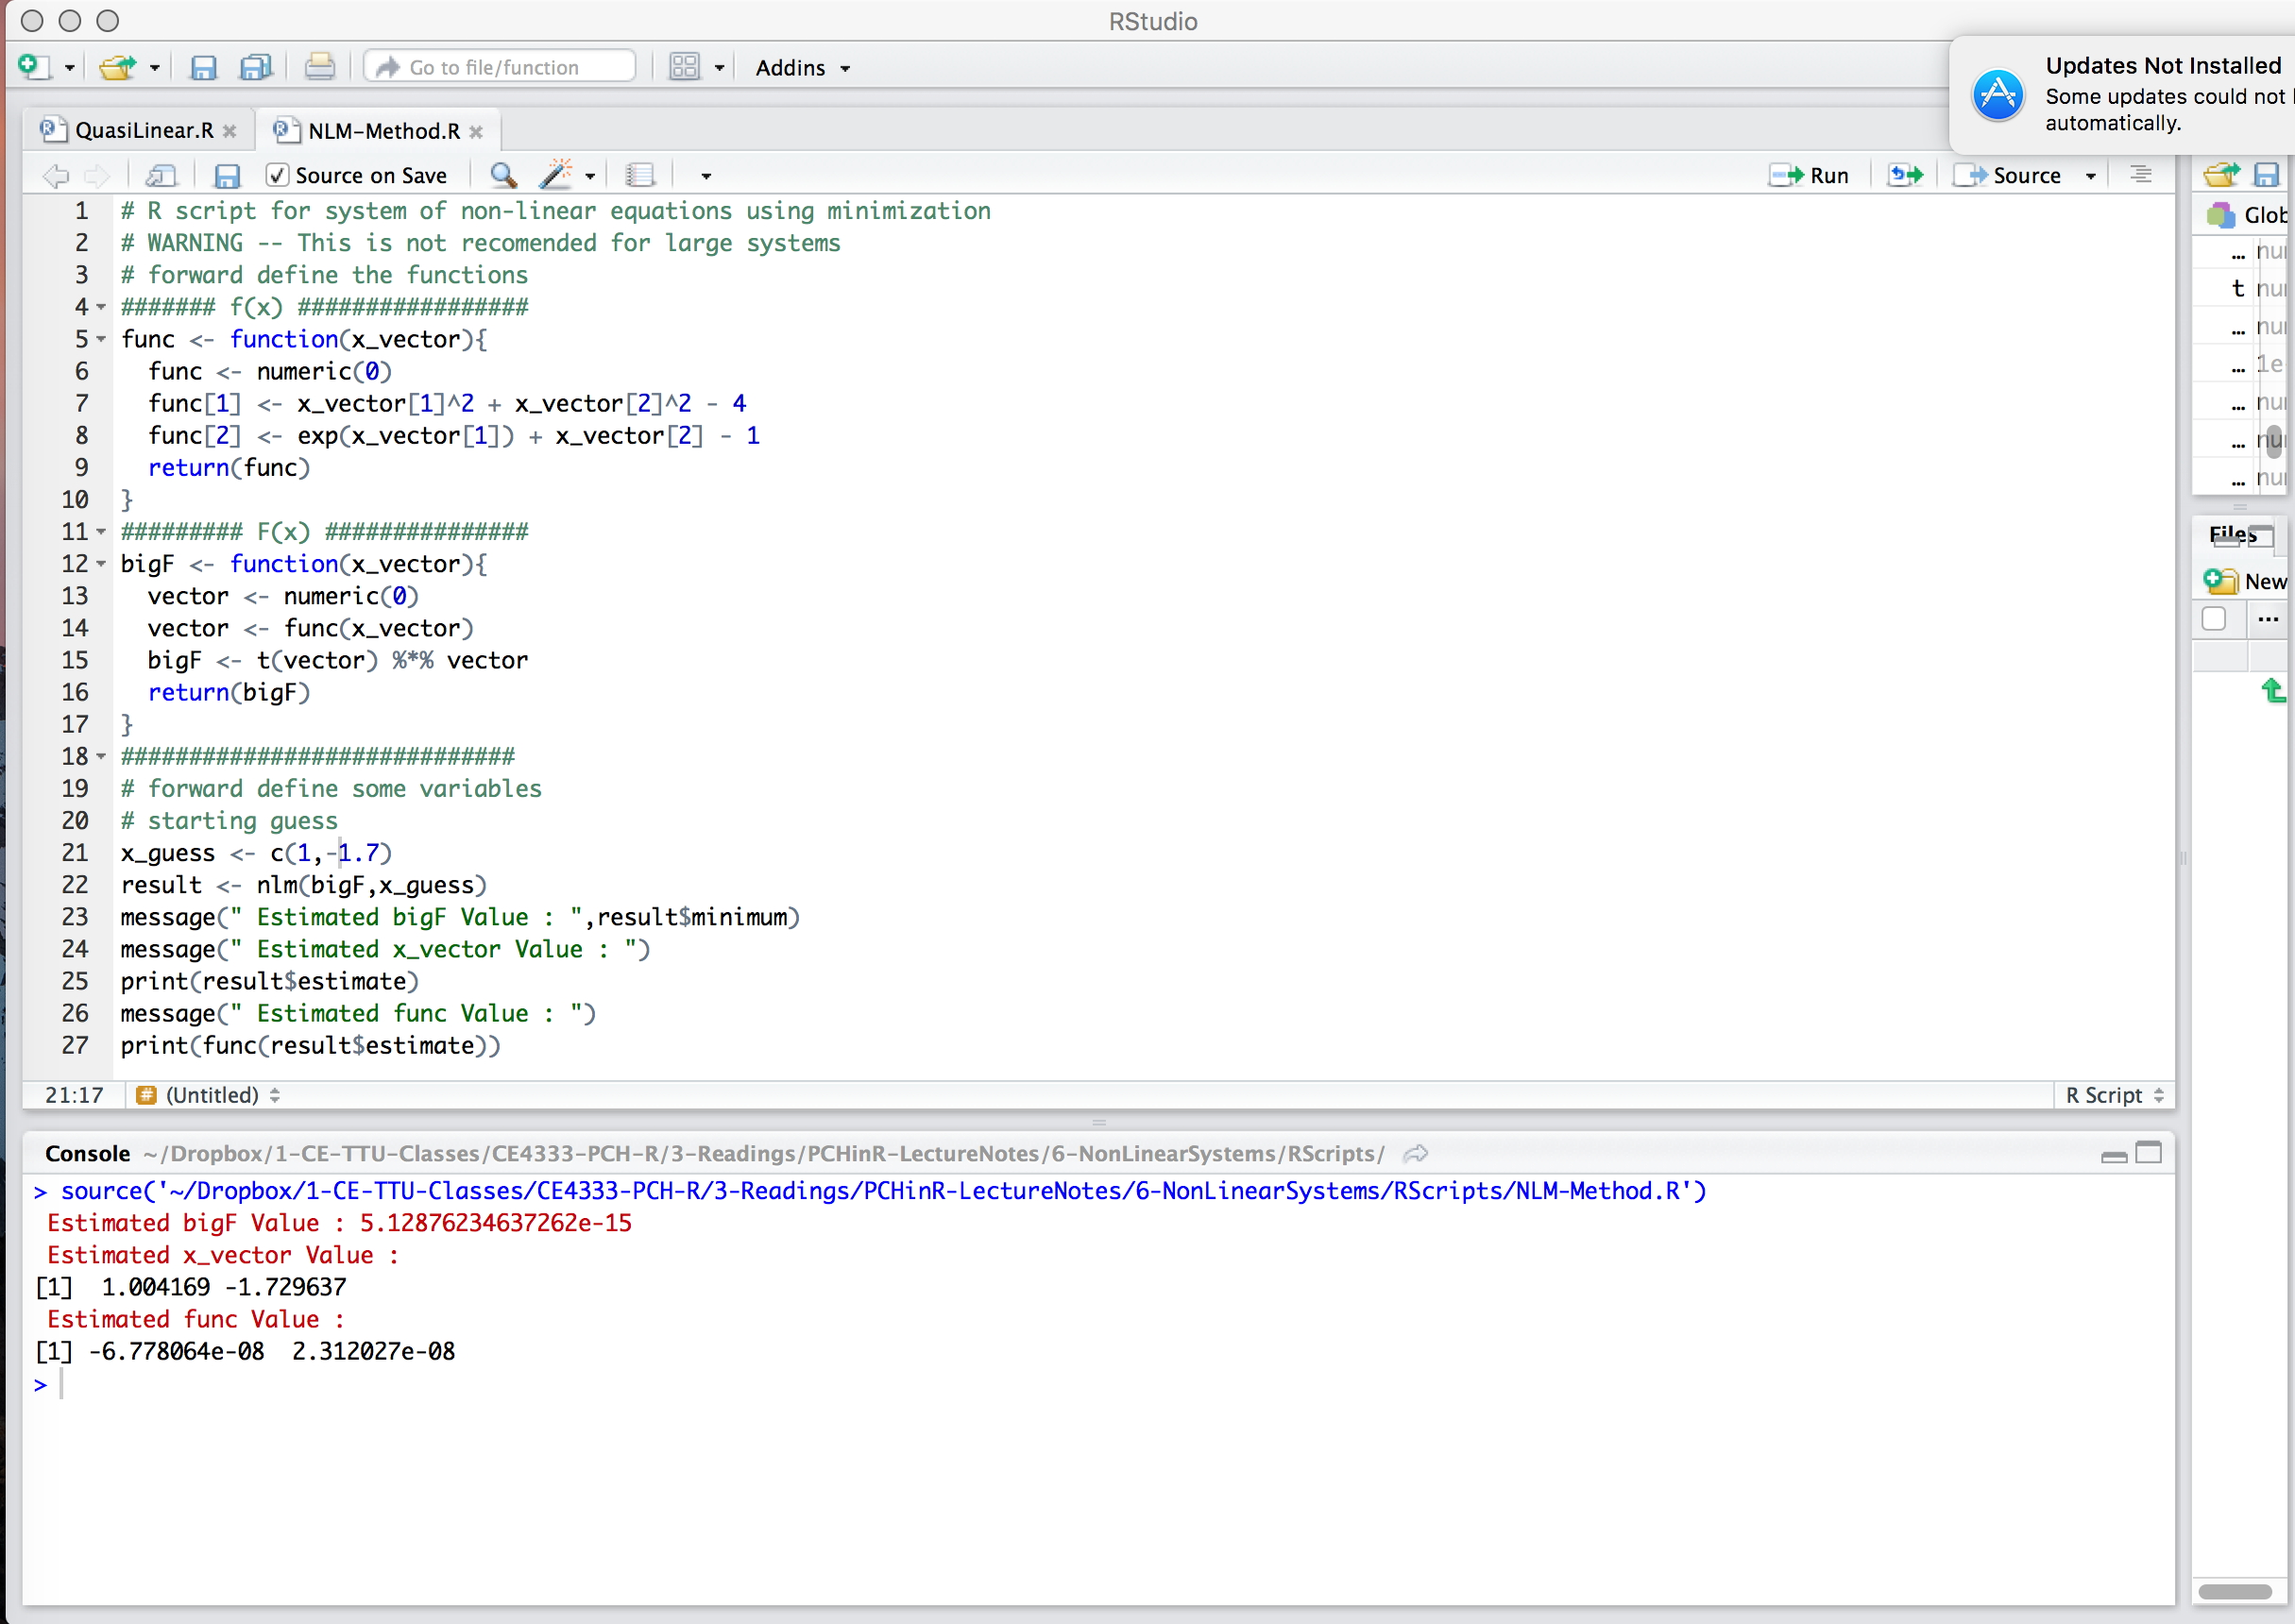
\includegraphics[height=4in]{./6-NonLinearSystems/NLM-Method-Works2.jpg} 
   \caption{Solution using \texttt{nlm(\dots)}.  Start vector (1.0,-1.7)}
   \label{fig:NLM-Method-Works2}
\end{figure}
\clearpage

\begin{figure}[h!] %  figure placement: here, top, bottom, or page
   \centering
   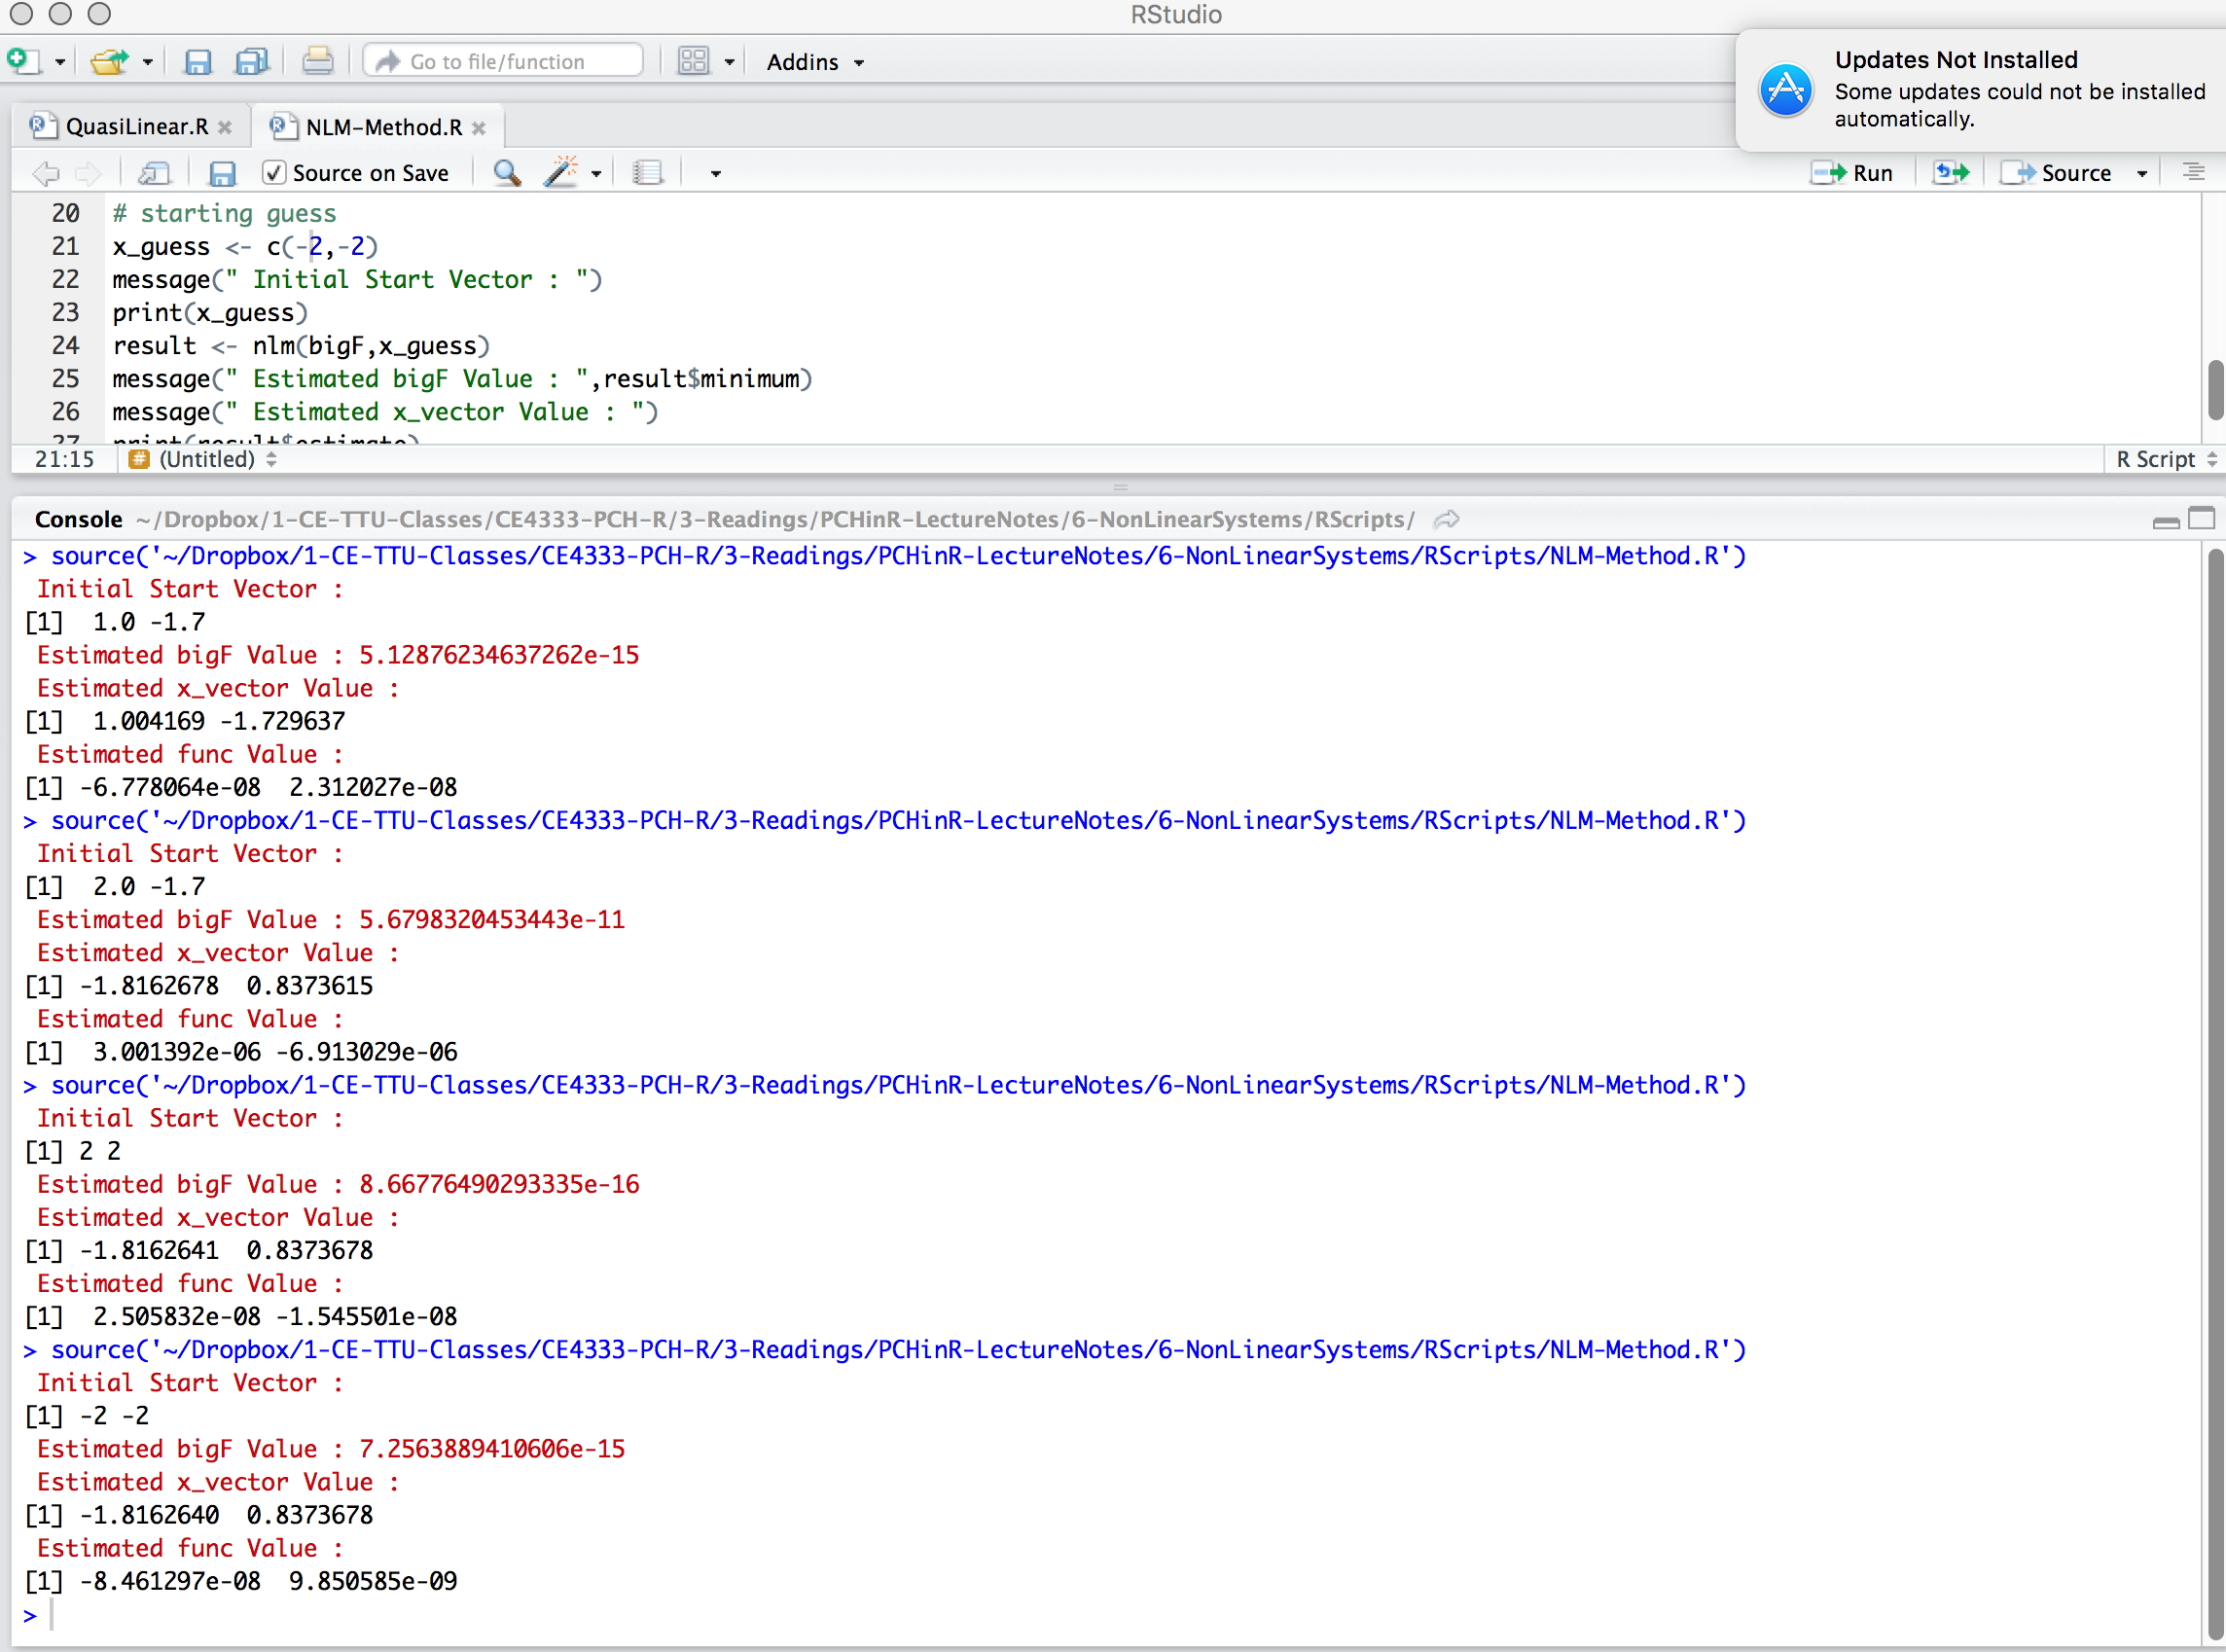
\includegraphics[width=6in]{./6-NonLinearSystems/NLM-Method-Works3.jpg} 
   \caption{Solution using \texttt{nlm(\dots)}.  Varying start vectors}
   \label{fig:NLM-Method-Works3}
\end{figure}

Using a non-linear minimization technique to solve systems of non-linear equations is not recommended for anything bigger than a few equations (maybe as many as 8 or 9).  
Quasi-linearization is a good technique --- the example here is intentionally pathological. 
The next chapter presents a better technique than quasi-linearization that can be used for large systems (assuming they will converge at all), and it is the method that will be used for pipeline networks.
%\newpage
%\subsection{Exercises}
%\begin{enumerate}
%\item Write a script that forward defines the multi-variate functions and implements the non-linear minimization technique in \textbf{R}.
%Implement the method and find a solution to:
%\begin{gather}
%\begin{matrix}
% x^3 & +~3y^2 & = 21\\
%x^2& +~2y  & = -2 \\
%\end{matrix}
%\end{gather}
%\item Write a script that forward defines the multi-variate functions and implements the non-linear minimization technique in \textbf{R}.
%Implement the method and find a solution to:
%\begin{gather}
%\begin{matrix}
%x^2 & +~ y^2 & +~z^2 & =~ 9\\
%~ & ~ & xyz & =~ 1\\
%x & +~ y & -z^2 & =~ 0\\
%\end{matrix}
%\end{gather}
%\item Write a script that forward defines the multi-variate functions and implements the non-linear minimization technique in \textbf{R}.
%Implement the method and find a solution to:
%\begin{gather}
%\begin{matrix}
%xyz & -~ x^2 & +~y^2 & =~ 1.34\\
%~ & xy &-~z^2 & =~ 0.09\\
%e^x & -~ e^y & +z & =~ 0.41\\
%\end{matrix}
%\end{gather}
%
%
%\end{enumerate}

